\documentclass{standalone}
\usepackage{tikz}
\begin{document}
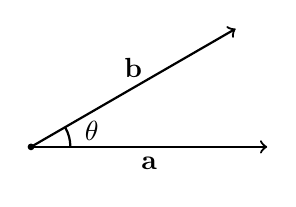
\begin{tikzpicture}
    % Draw the origin
    \coordinate (O) at (0,0);
    
    % Define the vectors
    \coordinate (A) at (3,0);  % Vector a
    \coordinate (B) at (30:3); % Vector b at 30 degrees
    
    % Draw the vectors
    \draw[->, thick] (O) -- (A) node[midway, below] {$\mathbf{a}$};
    \draw[->, thick] (O) -- (B) node[midway, above] {$\mathbf{b}$};
    
    % Draw the angle arc
    \draw[thick] (0.5,0) arc[start angle=0, end angle=30, radius=0.5];
    \node at (15:0.8) {$\theta$};
    
    % Add the origin point
    \filldraw (O) circle (1pt);
\end{tikzpicture}
\end{document}